\documentclass[11pt,aspectratio=169]{beamer}

\usetheme{Madrid}
\usecolortheme{seahorse}

\usepackage[utf8]{inputenc}
\usepackage{amsmath,amssymb}
\usepackage{algpseudocode}
\usepackage{algorithmicx}
\usepackage{xcolor}
\usepackage{listings}
\usepackage{booktabs}
\usepackage{tikz}

\setbeamertemplate{navigation symbols}{}
\setbeamertemplate{footline}[frame number]

\lstdefinestyle{py}{
  language=Python,
  basicstyle=\ttfamily\scriptsize,
  keywordstyle=\color{blue!70!black}\bfseries,
  commentstyle=\color{gray},
  stringstyle=\color{green!40!black},
  showstringspaces=false,
  breaklines=true,
  numbers=left,
  numberstyle=\tiny\color{gray},
  frame=single,
  xleftmargin=1.5em,
  aboveskip=0.3em,
  belowskip=0.3em
}

\title{Karatsuba Multiplication}
\subtitle{Fast Integer Multiplication via Divide and Conquer\\
\small Week 1 Supplement -- TOAE209/TOAH209: Design and Analysis of Algorithms}
\author{Foreign Trade University}
\date{}

\begin{document}

% ---------------------------------------------------------------
\begin{frame}
  \titlepage
\end{frame}
% ---------------------------------------------------------------

\begin{frame}{Outline}
  \tableofcontents
\end{frame}

% =================================================================
\section{Motivation}
% =================================================================

\begin{frame}{A question that sounds too simple to matter}
  \begin{block}{Question}
    How fast can we multiply two $n$-digit integers?
  \end{block}
  \vspace{0.5em}
  \begin{itemize}
    \item This is the algorithm you learned in \emph{grade school}: line up the digits,
    multiply, shift, add.
    \item It feels ``obviously'' as fast as multiplication can be.
    \item Yet in 1960, a 23-year-old student named \textbf{Anatoly Karatsuba}, in a seminar
    run by Andrey Kolmogorov, found a faster algorithm --- and disproved a conjecture that
    $\Theta(n^2)$ was optimal.
  \end{itemize}
  \vspace{0.5em}
  \begin{alertblock}{Why we care (course-wide theme)}
    This is our \textbf{first non-trivial divide-and-conquer algorithm}: it shows that
    ``obviously optimal'' brute force is often \emph{not} optimal, and that a clever
    recombination step can change the exponent in the running time, not just the constant.
  \end{alertblock}
\end{frame}

\begin{frame}{Where do large multiplications actually matter?}
  \begin{itemize}
    \item \textbf{Cryptography}: RSA works with numbers that have hundreds or thousands of
    digits (bits).
    \item \textbf{Computer algebra systems}: exact arbitrary-precision arithmetic
    (Python's \texttt{int}, Java's \texttt{BigInteger}).
    \item \textbf{Numerical / scientific computing}: high-precision constants ($\pi$ to
    trillions of digits), polynomial and matrix multiplication (same divide-and-conquer
    idea reused).
  \end{itemize}
  \vspace{1em}
  For \emph{small} numbers (say, 64-bit machine integers), the constant-factor overhead of
  Karatsuba is not worth it --- hardware multiplies those in $O(1)$. Karatsuba only pays off
  once $n$ (the number of digits) is large enough that the \emph{asymptotic} exponent
  dominates the constants. This is a recurring lesson: \emph{asymptotic analysis tells you
  what wins eventually, not what wins for every input size}.
\end{frame}

% =================================================================
\section{The Naive Algorithm and Its Cost}
% =================================================================

\begin{frame}{Grade-school multiplication, counted carefully}
  To multiply two $n$-digit numbers $x$ and $y$ by hand:
  \begin{itemize}
    \item Multiply $x$ by \emph{each} of the $n$ digits of $y$ separately $\Rightarrow$
    $n$ partial products.
    \item Each partial product costs $O(n)$ single-digit multiplications (with carries).
    \item Add up the $n$ shifted partial products: $O(n)$ more work per addition, $O(n)$
    additions.
  \end{itemize}
  \[
    \underbrace{n}_{\text{partial products}} \times \underbrace{O(n)}_{\text{cost each}}
    \;=\; \Theta(n^2) \text{ single-digit multiplications.}
  \]
  \begin{exampleblock}{Key fact}
    The grade-school algorithm is $\boxed{\Theta(n^2)}$. Doubling the number of digits
    quadruples the work.
  \end{exampleblock}
  \textbf{Question this section answers:} can we multiply two $n$-digit numbers using
  asymptotically \emph{fewer} than $\Theta(n^2)$ single-digit multiplications?
\end{frame}

% =================================================================
\section{Divide and Conquer: The Idea}
% =================================================================

\begin{frame}{Step 1: split each number in half}
  Let $x$ and $y$ be $n$-digit numbers (assume $n$ is even; pad with a leading zero if not).
  Split each into a high half and a low half, each with $n/2$ digits:
  \[
    x = x_1 \cdot 10^{n/2} + x_0, \qquad y = y_1 \cdot 10^{n/2} + y_0.
  \]
  \begin{center}
  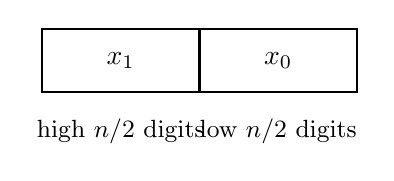
\begin{tikzpicture}[scale=1]
    \draw[thick] (0,0) rectangle (2,0.8);
    \draw[thick] (2,0) rectangle (4,0.8);
    \node at (1,0.4) {$x_1$};
    \node at (3,0.4) {$x_0$};
    \node at (1,-0.5) {\small high $n/2$ digits};
    \node at (3,-0.5) {\small low $n/2$ digits};
  \end{tikzpicture}
  \end{center}
  \textbf{Example:} $x = 1234$, $n = 4$, $n/2 = 2$ $\Rightarrow$ $x_1 = 12$, $x_0 = 34$, and
  indeed $12 \cdot 10^2 + 34 = 1234$. $\checkmark$
\end{frame}

\begin{frame}{Step 2: expand the product}
  Multiply out $xy = (x_1 \cdot 10^{n/2} + x_0)(y_1 \cdot 10^{n/2} + y_0)$:
  \[
    xy = \underbrace{x_1 y_1}_{z_2} \cdot 10^{n} \;+\; \underbrace{(x_1y_0 + x_0y_1)}_{z_1}
    \cdot 10^{n/2} \;+\; \underbrace{x_0 y_0}_{z_0}.
  \]
  This expresses the product of two $n$-digit numbers in terms of products of
  \textbf{$n/2$-digit} numbers: $x_1y_1$, $x_1y_0$, $x_0y_1$, $x_0y_0$.
  \vspace{1em}
  \begin{alertblock}{The naive divide-and-conquer attempt}
    Compute all \textbf{four} products $x_1y_1,\ x_1y_0,\ x_0y_1,\ x_0y_0$ recursively, then
    combine with shifts and additions (which cost only $O(n)$).
  \end{alertblock}
\end{frame}

\begin{frame}{Why four recursive calls is \emph{not} good enough}
  Let $T(n)$ be the number of single-digit multiplications to multiply two $n$-digit
  numbers this way. Four recursive calls on half-size inputs, plus $O(n)$ combination work:
  \[
    T(n) = 4\, T(n/2) + O(n).
  \]
  By the Master theorem ($a = 4$, $b = 2$, $\log_b a = \log_2 4 = 2$):
  \[
    T(n) = \Theta(n^2).
  \]
  \begin{alertblock}{No improvement!}
    Splitting the numbers in half and recursing on \textbf{four} sub-products gives back
    exactly the same $\Theta(n^2)$ bound as grade-school multiplication. Divide and conquer,
    by itself, bought us nothing here --- \emph{something smarter is needed}.
  \end{alertblock}
\end{frame}

% =================================================================
\section{Karatsuba's Trick}
% =================================================================

\begin{frame}{The key idea: trade a multiplication for additions}
  We do not need $x_1y_0$ and $x_0y_1$ \emph{individually} --- only their \textbf{sum}
  $z_1 = x_1y_0 + x_0y_1$. Karatsuba's observation:
  \[
    (x_1 + x_0)(y_1 + y_0) = x_1y_1 + x_1y_0 + x_0y_1 + x_0y_0.
  \]
  Rearranging gives the cross term $x_1y_0 + x_0y_1$ directly:
  \begin{block}{Karatsuba's identity}
    \[
      z_1 = x_1y_0 + x_0y_1 = \underbrace{(x_1+x_0)(y_1+y_0)}_{\text{one new product}} -
      \underbrace{x_1y_1}_{z_2} - \underbrace{x_0y_0}_{z_0}.
    \]
  \end{block}
  We already need to compute $z_2 = x_1y_1$ and $z_0 = x_0y_0$ for the other terms of the
  product. So $z_1$ costs \textbf{one extra multiplication} --
  $(x_1+x_0)(y_1+y_0)$ -- plus a few $O(n)$ additions/subtractions, \emph{instead of} the
  two multiplications $x_1y_0$ and $x_0y_1$.
\end{frame}

\begin{frame}{From four multiplications down to three}
  \begin{center}
  \begin{tabular}{@{}lll@{}}
    \toprule
    & Naive divide \& conquer & Karatsuba \\
    \midrule
    Recursive products & $x_1y_1,\ x_1y_0,\ x_0y_1,\ x_0y_0$ & $x_1y_1,\ x_0y_0,\ (x_1{+}x_0)(y_1{+}y_0)$ \\
    Count & 4 & \textbf{3} \\
    \bottomrule
  \end{tabular}
  \end{center}
  \vspace{1em}
  Given the three products $z_2 = x_1y_1$, $z_0 = x_0y_0$, and
  $p = (x_1+x_0)(y_1+y_0)$, recover $z_1$ and assemble the answer:
  \[
    z_1 = p - z_2 - z_0, \qquad
    xy = z_2 \cdot 10^{n} + z_1 \cdot 10^{n/2} + z_0.
  \]
  All the additions, subtractions, and shifts (multiplying by a power of $10$) cost only
  $O(n)$ total. \textbf{Only three multiplications of half-size numbers are ever needed.}
\end{frame}

% =================================================================
\section{Recurrence and Running Time}
% =================================================================

\begin{frame}{Solving the recurrence}
  Karatsuba's algorithm makes \textbf{3} recursive calls on inputs of size $n/2$, plus
  $O(n)$ work to form the sums $(x_1+x_0)$, $(y_1+y_0)$ and to combine results:
  \[
    T(n) = 3\,T(n/2) + O(n), \qquad T(1) = O(1).
  \]
  By the \textbf{Master theorem} with $a = 3$, $b = 2$, $f(n) = O(n)$:
  \[
    \log_b a = \log_2 3 \approx 1.585 \quad > \quad 1 = \deg f(n)
  \]
  so we are in the ``recursion dominates'' case, giving
  \[
    \boxed{T(n) = \Theta\!\left(n^{\log_2 3}\right) \approx \Theta(n^{1.585}).}
  \]
  \begin{alertblock}{Why this matters}
    $n^{1.585}$ grows \emph{strictly slower} than $n^2$. For $n = 1024$ digits,
    $n^2 \approx 1.05 \times 10^6$ while $n^{1.585} \approx 3.2\times10^4$ --- roughly
    \textbf{30$\times$ fewer} single-digit multiplications.
  \end{alertblock}
\end{frame}

\begin{frame}{Recursion tree intuition}
  \begin{center}
  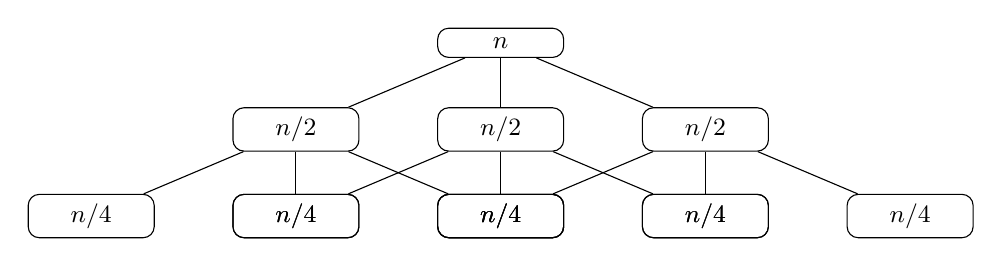
\begin{tikzpicture}[level distance=1.1cm, sibling distance=2.6cm,
      every node/.style={draw, rounded corners, minimum width=1.6cm, align=center, font=\small}]
    \node {$n$}
      child { node {$n/2$}
        child { node {$n/4$} }
        child { node {$n/4$} }
        child { node {$n/4$} }
      }
      child { node {$n/2$}
        child { node {$n/4$} }
        child { node {$n/4$} }
        child { node {$n/4$} }
      }
      child { node {$n/2$}
        child { node {$n/4$} }
        child { node {$n/4$} }
        child { node {$n/4$} }
      };
  \end{tikzpicture}
  \end{center}
  \begin{itemize}
    \item Branching factor $3$ (not $4$): each level has $3^k$ nodes of size $n/2^k$.
    \item Work per node is $O(\text{node size})$, so level $k$ costs
    $3^k \cdot O(n/2^k) = O(n) \cdot (3/2)^k$.
    \item Levels \emph{grow geometrically} ($3/2 > 1$), so the \textbf{last level}
    (about $\log_2 n$ levels down, $n^{\log_2 3}$ leaves) dominates the total ---
    exactly what the Master theorem tells us algebraically.
  \end{itemize}
\end{frame}

% =================================================================
\section{Worked Running Example}
% =================================================================

\begin{frame}{Running example: $1234 \times 5678$}
  Let $x = 1234$, $y = 5678$, so $n = 4$ and $n/2 = 2$.
  \begin{align*}
    x_1 &= 12, & x_0 &= 34, \\
    y_1 &= 56, & y_0 &= 78.
  \end{align*}
  \textbf{Step 1 -- two ``easy'' recursive products:}
  \[
    z_2 = x_1 y_1 = 12 \times 56 = 672, \qquad
    z_0 = x_0 y_0 = 34 \times 78 = 2652.
  \]
  \textbf{Step 2 -- the one ``clever'' recursive product:}
  \[
    x_1 + x_0 = 46, \qquad y_1 + y_0 = 134, \qquad
    p = 46 \times 134 = 6164.
  \]
\end{frame}

\begin{frame}{Running example (continued): combine}
  \textbf{Step 3 -- recover the cross term:}
  \[
    z_1 = p - z_2 - z_0 = 6164 - 672 - 2652 = 2840.
  \]
  \textbf{Step 4 -- assemble the final answer:}
  \[
    xy = z_2 \cdot 10^{4} + z_1 \cdot 10^{2} + z_0
       = 672\,{\times}\,10000 \;+\; 2840\,{\times}\,100 \;+\; 2652.
  \]
  \[
    xy = 6{,}720{,}000 \;+\; 284{,}000 \;+\; 2{,}652 \;=\; \boxed{7{,}006{,}652}.
  \]
  \begin{exampleblock}{Sanity check}
    Direct multiplication: $1234 \times 5678 = 7{,}006{,}652$. \checkmark~Matches exactly,
    using only \textbf{three} multiplications of 2-digit numbers instead of four.
  \end{exampleblock}
  Each of $z_2$, $z_0$, and $p$ above would themselves be computed recursively by the same
  method once the numbers are large; here they are small enough to read off directly (the
  recursion's base case).
\end{frame}

% =================================================================
\section{Algorithm and Python Implementation}
% =================================================================

\begin{frame}{Pseudocode}
  \begin{algorithmic}[1]
    \Function{Karatsuba}{$x$, $y$}
      \If{$x < 10$ \textbf{or} $y < 10$} \Comment{base case}
        \State \Return $x \cdot y$
      \EndIf
      \State $n \gets \max(\textsc{NumDigits}(x), \textsc{NumDigits}(y))$
      \State $m \gets \lceil n/2 \rceil$
      \State $x_1, x_0 \gets \lfloor x / 10^m \rfloor,\ x \bmod 10^m$
      \State $y_1, y_0 \gets \lfloor y / 10^m \rfloor,\ y \bmod 10^m$
      \State $z_2 \gets \Call{Karatsuba}{x_1, y_1}$
      \State $z_0 \gets \Call{Karatsuba}{x_0, y_0}$
      \State $p \gets \Call{Karatsuba}{x_1+x_0,\ y_1+y_0}$
      \State $z_1 \gets p - z_2 - z_0$
      \State \Return $z_2 \cdot 10^{2m} + z_1 \cdot 10^{m} + z_0$
    \EndFunction
  \end{algorithmic}
\end{frame}

\begin{frame}[fragile]{Python implementation}
  \begin{lstlisting}[style=py]
def karatsuba(x: int, y: int) -> int:
    # Base case: single-digit multiplication.
    if x < 10 or y < 10:
        return x * y

    n = max(len(str(x)), len(str(y)))
    m = n // 2                     # split point (use ceil for odd n)
    if n % 2:
        m += 1

    high_x, low_x = divmod(x, 10 ** m)
    high_y, low_y = divmod(y, 10 ** m)

    z2 = karatsuba(high_x, high_y)          # x1 * y1
    z0 = karatsuba(low_x, low_y)            # x0 * y0
    p  = karatsuba(high_x + low_x,
                   high_y + low_y)          # (x1+x0)(y1+y0)
    z1 = p - z2 - z0                        # x1*y0 + x0*y1

    return z2 * 10 ** (2 * m) + z1 * 10 ** m + z0
  \end{lstlisting}
\end{frame}

\begin{frame}[fragile]{Testing it against the running example}
  \begin{lstlisting}[style=py]
>>> karatsuba(1234, 5678)
7006652
>>> 1234 * 5678
7006652
>>> karatsuba(1234, 5678) == 1234 * 5678
True

>>> import random
>>> all(karatsuba(a, b) == a * b
...     for a, b in ((random.randint(0, 10**50),
...                   random.randint(0, 10**50))
...                  for _ in range(1000)))
True
  \end{lstlisting}
  \vspace{0.5em}
  This is exactly the spirit of \textbf{Problem 15} in this week's practical exercises:
  implement Karatsuba, then instrument it (count single-digit multiplications) and compare
  against the naive $\Theta(n^2)$ algorithm as $n$ grows.
\end{frame}

% =================================================================
\section{Comparing the Two Algorithms}
% =================================================================

\begin{frame}{Naive vs.\ Karatsuba: growth of single-digit multiplications}
  \begin{center}
  \begin{tabular}{@{}rrrr@{}}
    \toprule
    Digits $n$ & Naive $\Theta(n^2)$ & Karatsuba $\Theta(n^{1.585})$ & Speedup \\
    \midrule
    $10$    & $100$                & $\approx 39$                & $2.6\times$ \\
    $100$   & $10{,}000$           & $\approx 1{,}555$           & $6.4\times$ \\
    $1{,}000$ & $1{,}000{,}000$    & $\approx 61{,}824$          & $16\times$ \\
    $10{,}000$ & $100{,}000{,}000$ & $\approx 2{,}459{,}942$     & $41\times$ \\
    \bottomrule
  \end{tabular}
  \end{center}
  \vspace{1em}
  \begin{itemize}
    \item The gap \emph{widens} as $n$ grows -- exactly what ``different exponent'' means.
    \item In practice, real libraries (e.g., Python's \texttt{int}, GMP) switch from
    schoolbook multiplication to Karatsuba once operands exceed a threshold (tens of
    digits), and to even faster methods (Toom--Cook, Sch\"onhage--Strassen, using FFTs) for
    very large operands -- the same divide-and-conquer philosophy, pushed further.
  \end{itemize}
\end{frame}

% =================================================================
\section{Summary}
% =================================================================

\begin{frame}{Summary}
  \begin{enumerate}
    \item Grade-school multiplication of $n$-digit numbers is $\Theta(n^2)$.
    \item Splitting numbers in half and recursing on all \textbf{4} cross-products
    (naive divide and conquer) is \emph{still} $\Theta(n^2)$ -- splitting alone is not
    enough.
    \item Karatsuba's identity
    $x_1y_0 + x_0y_1 = (x_1{+}x_0)(y_1{+}y_0) - x_1y_1 - x_0y_0$
    trades two multiplications for one multiplication plus $O(n)$ extra additions, cutting
    the branching factor from $4$ to \textbf{3}.
    \item The recurrence $T(n) = 3T(n/2) + O(n)$ solves to
    $\Theta(n^{\log_2 3}) \approx \Theta(n^{1.585})$, asymptotically better than
    $\Theta(n^2)$.
    \item This is our first concrete example that \textbf{divide-and-conquer is not
    automatically better} -- the \emph{combine} step must be designed cleverly (fewer
    recursive calls, not just smaller ones).
  \end{enumerate}
  \vspace{0.5em}
  \begin{alertblock}{Looking ahead}
    We revisit divide-and-conquer formally, with the Master theorem proved in full, in
    Weeks 6--7. Karatsuba is the template: split, recurse, and find a combine step that
    minimizes the number of recursive calls.
  \end{alertblock}
\end{frame}

\end{document}
